\documentclass{article}
\usepackage{graphicx}
\usepackage{url}
\usepackage{amsmath}
\usepackage{amssymb}
\usepackage{amsthm}
\usepackage{multirow}
\usepackage{mathtools}
\usepackage{algorithm}
\usepackage[noend]{algpseudocode}
\usepackage{xcolor}
\usepackage{sansmath}   % i matematika u boksu je bezserifna, kao na uzoru
\usepackage[skins,breakable]{tcolorbox}

%============================ izgled okvira ==================================
\definecolor{blokbg}{RGB}{221,221,246}

\newtcolorbox{algbox}[1]{%
  enhanced, breakable,
  colback=blokbg, colframe=blokbg, colbacktitle=blokbg, coltitle=black,
  boxrule=0pt, arc=3mm, titlerule=0pt, boxsep=1mm,
  left=3mm, right=3mm, top=2mm, bottom=3mm, toptitle=1mm, bottomtitle=0mm,
  drop shadow=black!40,
  fonttitle=\sffamily\sansmath, fontupper=\sffamily\sansmath,
  title={\textbf{Algoritam:}\ #1}%
}

\newtcolorbox{structbox}[1]{%
  enhanced, breakable,
  colback=blokbg, colframe=blokbg, colbacktitle=blokbg, coltitle=black,
  boxrule=0pt, arc=3mm, titlerule=0pt, boxsep=1mm,
  left=3mm, right=3mm, top=2mm, bottom=3mm, toptitle=1mm, bottomtitle=0mm,
  drop shadow=black!40,
  fonttitle=\sffamily\sansmath, fontupper=\sffamily\sansmath,
  title={\textbf{Struktura:}\ #1}%
}

%======================= srpske klju\v cne re\v ci u pseudokodu ====================
\algrenewcommand\algorithmicif{\textbf{ako je}}
\algrenewcommand\algorithmicthen{\textbf{onda}}
\algrenewcommand\algorithmicelse{\textbf{ina\v ce}}
\algrenewcommand\algorithmicfor{\textbf{za}}
\algrenewcommand\algorithmicforall{\textbf{za svaki}}
\algrenewcommand\algorithmicdo{\textbf{radi}}
\algrenewcommand\algorithmicwhile{\textbf{dok je}}
\algrenewcommand\algorithmicreturn{\textbf{vrati}}
% komentari u viti\v castim zagradama, kao na uzoru
\algrenewcommand\algorithmiccomment[1]{\quad\{#1\}}

%=== \LState: kao \State, ali se prelom reda poravnava sa po\v cetkom teksta ====
\makeatletter
\newcommand{\LState}[1]{\State\parbox[t]{\dimexpr\linewidth-\ALG@tlm\relax}{#1\strut}}
\makeatother

%============================ pomo\' cne skra\' cenice =============================
\newcommand{\Proc}[1]{\textsf{#1}}                     % ime procedure
\newcommand{\Fld}[2]{#1.\text{\sffamily\itshape #2}}  % polje doga\dj aja: e.end, ...
\newcommand{\Tru}{\textbf{true}}
\newcommand{\Fls}{\textbf{false}}


\DeclareMathOperator*{\argmax}{arg\,max}
\DeclareMathOperator*{\argmin}{arg\,min}

\usepackage[OT2, OT1]{fontenc}
\usepackage[english, serbian]{babel}



\newtheorem{teorema}{Teorema}[section]
\newtheorem{lema}{Lema}[section]
\newtheorem{definicija}{Definicija}[section]
\newtheorem{primer}{Primer}[section]

\title{Izračunavanje i vizuelizacija poligona vidljivosti}
\author{Tijana Jak\v si\' c}
\date{14. septembar 2024.}

\begin{document}
\renewcommand{\contentsname}{Sadr\v zaj}

\maketitle
\thispagestyle{empty} 
\tableofcontents

\newpage
\pagenumbering{arabic}


\section{Uvod}
Ukoliko je data mapa ravni posmatrane odozgo sa nekim preprekama u vidu segmenata, i tačka posmatranja $p$, poligon vidljivosti predstavlja podskup te ravni koji opisuje sve tačke vidljive iz $p$. 

\begin{figure}[htp]
    \centering
    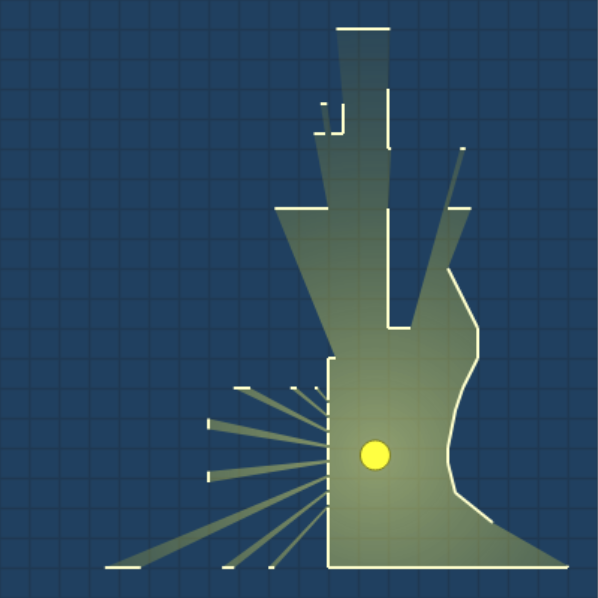
\includegraphics[height=5cm]{visibility_in_darkness.png}
    \caption{Ilustracija vidljivog regiona iz date tačke \cite{redblob}}
    \label{darkness}
\end{figure}

Poligon vidljivosti ima veze sa poznatim problemom umetničke galerije, a nalazi praktičnu primenu u video igrama, robotici i navigaciji.

Prvi rad koji opisuje pronala\v zenje poligona vidljivosti primenom tehnike rotacionog bri\v su\' ceg zraka je \cite{asano}.
Ovaj projekat implementira sli\v can algoritam u programskom jeziku C++, oslanjaju\' ci se na biblioteku SFML radi vizuelizacije. 
Implementirana je interaktivna vizuelizacija u kojoj korisnik položajem miša zadaje koordinate tački posmatranja. 
Osim toga, mogu\' ce je zadati koordinate preprekama, menjanjem fajla \texttt{segments.txt} pre pokretanja programa.

\section{Definicija problema}

Matematički, poligon vidljivosti se može uvesti na sledeći način:
Neka su u ravni $\mathbf{R}^2$ dati skup duži $S$ (\textit{prepreke}) i tačka $p$ koja se ne nalazi na nekoj od prepreka. Poligon vidljivosti $V$ je tada skup tačaka $q$ u $\mathbf{R}^2$ takvih da segment $pq$ nema preseka ni sa jednom preprekom. 

\begin{figure}[htp]
    \centering
    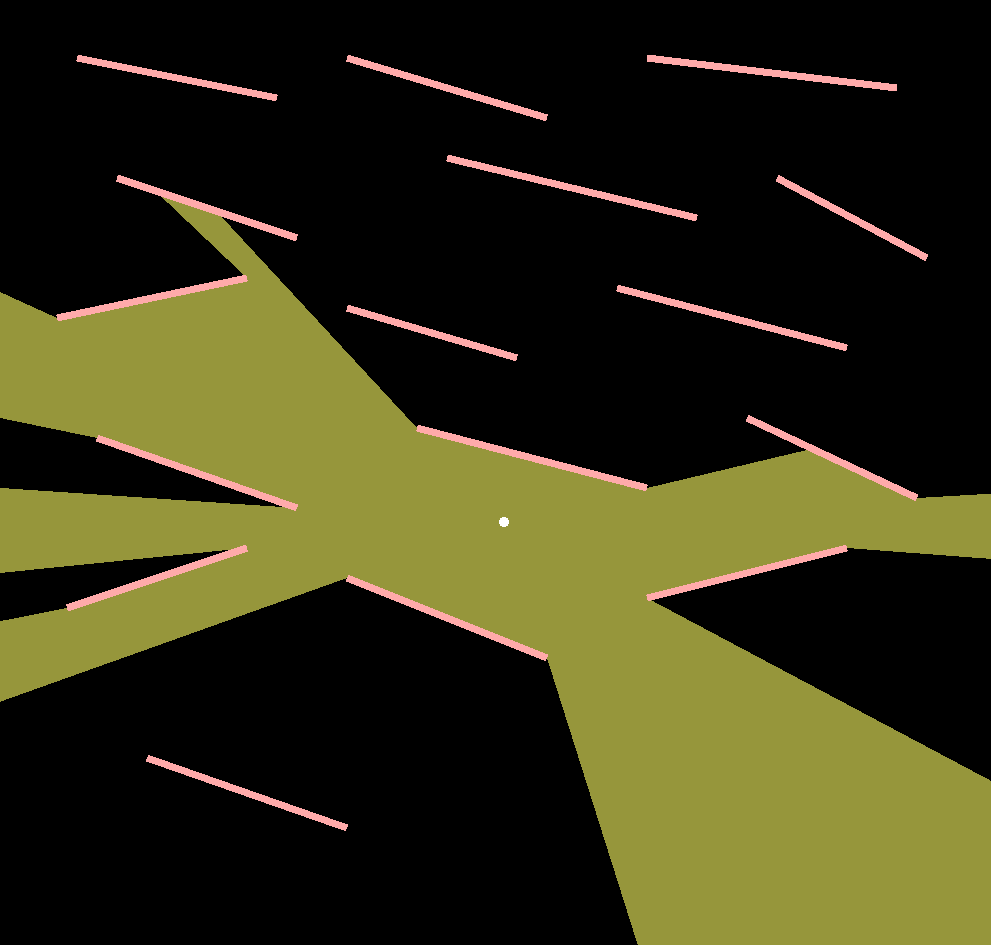
\includegraphics[height=5cm]{Screenshot From 2026-09-14 16-55-28.png}
    \caption{Poligon vidljivosti }
    \label{poligon}
\end{figure}

Primetimo da ovako definisan, poligon vidljivosti može biti neograničen podskup ravni. Prva dodatna pretpostavka koja se pravi radi implementacije jeste da je skup $S$ kona\v can. Dalje pretpostavljamo da ne radimo sa celom ravni, već da su u skupu prepreka dati segmenti koji prave zatvorenu regiju u kojoj se svi ostali segmenti i ta\v cka posmatranja nalaze. Ovo je u redu jer je bilo kom kona\v cnom skupu segmenata moguće naknadno dodati granicu.

Osim toga, pretpostavlja se da  se datim segmentima ne seku unutrašnjosti. U slučaju datih duži koje imaju preseke u unutrašnjim tačkama, bilo bi potrebno preprocesirati ulazni skup du\v zi, ali u ovom projektu to nije implementirano.

Dakle, algoritam za ulaz prima skup prepreka i tačku posmatranja koji zadovoljavaju sledeće preptostavke:
\begin{itemize}
    \item Prepreke su segmenti kojima se unutrašnjosti ne presecaju
    \item Postoji podskup segmenata koji čini zatvorenu regiju, u kojoj se nalaze svi ostali segmenti i ta\v cka posmatranja
\end{itemize}

Kao izlaz, algoritam daje vektor tačaka koji opisuje poligon vidljivosti.


\section{Implementacija}

\subsection{Strukture podataka}

Pomo\' cne geometrijske strukture podataka:
\begin{structbox}{\Proc{Point}}
\begin{algorithmic}
        \State $x$: float
        \State $y$: float
\end{algorithmic}
\end{structbox}

\begin{structbox}{\Proc{Segment}}
\begin{algorithmic}
        \State $a$: Point
        \State $b$: Point
\end{algorithmic}
\end{structbox}

Struktura podataka koja opisuje doga\dj aj:

\begin{structbox}{\Proc{Event}}
\begin{algorithmic}
        \State $point$: Point
        \State $segment$: Segment
        \State $end$: bool
\end{algorithmic}
\end{structbox}

Atribut $end$ čuva informaciju o tome  da li je $point$ po\v cetno ili krajnje teme segmenta. Ovo se može utvrditi na osnovu orijentacije trougla $(p, segment.a, segment.b)$.
\subsubsection{Kontejnerske strukture podataka}
\textbf{Red doga\dj aja.} Doga\dj aji su sme\v stani u vektor $\mathcal{E}$. Kako je za tehniku bri\v su\' ceg zraka potrebno sortirati doga\dj aje, uveden je komparator doga\dj aja \Proc{CompareEvents}. 
Glavni kriterijum je ugao vektora $p \to e.point$. Ukoliko ima vi\v se doga\dj aja na istom zraku posmatranja, ova implementacija tretira udaljenije doga\dj aje kao manje, potom ako su identi\v cni i ugao i udaljenost, tretira $end$ doga\dj aje kao manje.

\textbf{Status.} Status je struktura podataka $\mathcal{T}$ koja treba da \v cuva niz du\v zi koje seku rotacioni bri\v su\' ci zrak, ispravno pore\dj an tako da $\min\mathcal{T}$ predstavlja prvi vidljiv segment. Osim toga, $\mathcal{T}$ treba da omogu\' cava efikasnu pretragu, umetanje i brisanje elemenata. Zato se koristi ure\dj eno balansirano binarno stablo. Uveden je komparator \Proc{CompareSegments} koji opisuje relaciju ,,ispred``. Relacija zavisi od ta\v cke posmatranja $p$. Primetimo da relacija ispred nije isto \v sto i relacija udaljenosti od $p$.

\begin{figure}[htp]
    \centering
    
\includegraphics[height=5cm]{primer.png}
    \caption{Dva segmenta kojima se relacija ispred ne poklapa sa udaljeno\v s\' cu od $p$}
    \label{primer}
\end{figure}

Za segment $s_1$ va\v zi da je ispred segmenta $s_2$ ukoliko postoji zrak posmatranja $r$ iz ra\v cke posmatranja $p$ koji se\v ce oba segmenta i, ukoliko su ti preseci $I_1$ i $I_2$, va\v zi $d(I_1, p) < d(I_2, p)$. Drugim re\v cima, ukoliko je udaljenost do ta\v cke posmatranja du\v z zrak posmatranja manja. Upravo zbog ovoga je va\v zno da se datim segmentima ne seku unutra\v snjosti - da bi ova relacija bila doro definisana.

\subsection{Algoritam}

U nastavku je opisan glavni algoritam, koji kao ulaz prima tačku posmatranja $p$ i skup segmenata prepreka $\mathcal{S}$, a kao izlaz vraća vektor čvorova poligona vidljivosti $\mathcal{V}$.

\begin{algbox}{\Proc{VisibilityPolygon}$(p, \mathcal{S})$}
\begin{algorithmic}[1]
  \State Inicijalizuj prazan vektor doga\dj aja $\mathcal{E}$
  \ForAll{segment $s$ u $\mathcal{S}$}
    \LState{Za svaki \v cvor segmenta $s$ dodaj odgovaraju\' ci doga\dj aj
            u $\mathcal{E}$}
  \EndFor
  \State Sortiraj $\mathcal{E}$ po kriterijumu \Proc{CompareEvents}
  \State Inicijalizuj praznu strukturu za status $\mathcal{T}$
  \State Inicijalizuj prazan vektor $\mathcal{V}$
  \ForAll{$e$ u $\mathcal{E}$}
    \State \Proc{ProcessEvent}$(e)$
  \EndFor
\end{algorithmic}
\end{algbox}

Dalje je opisan algoritam obrade doga\dj aja, koji za ulaz prima doga\dj aj $e$, 
i na osnovu toga inkrementalno a\v zurira $\mathcal{V}$. Ugao posmatranja je ugao koji formira vektor $p \to e.point$, a zrak posmatranja poluprava koja polazi iz $p$ i ima ugao posmatranja.
\begin{algbox}{\Proc{ProcessEvent}$(e)$}
\begin{algorithmic}[1]
  \State A\v zuriraj ugao posmatranja
  \If{$\Fld{e}{end} = \Tru$}
    \State Obri\v si $\Fld{e}{segment}$ iz $\mathcal{T}$
    \If{$\Fld{e}{segment} = \min(\mathcal{T})$}
         \Comment{segment je bio vidljiv}
      \State Dodaj $\Fld{e}{point}$ u $\mathcal{V}$
      \If{$\mathcal{T} \neq \emptyset$}
        \LState{Dodaj u $\mathcal{V}$ presek novog $\min(\mathcal{T})$ sa zrakom
                posmatranja}
      \EndIf
    \EndIf
  \Else \Comment{$\Fld{e}{end} = \Fls$}
    \If{$\mathcal{T} \neq \emptyset$}
      \LState{Prona\dj i ta\v cku $q$ preseka $\min(\mathcal{T})$ sa zrakom
              posmatranja}
    \EndIf
    \State Dodaj $\Fld{e}{segment}$ u $\mathcal{T}$
    \If{$\Fld{e}{segment} = \min(\mathcal{T})$}
         \Comment{novi najbli\v zi segment}
      \If{ta\v cka $q$ je prona\dj ena}
        \State Dodaj $q$ u $\mathcal{V}$
      \EndIf
      \State Dodaj $\Fld{e}{point}$ u $\mathcal{V}$
    \EndIf
  \EndIf
\end{algorithmic}
\end{algbox}

\section{Analiza slo\v zenosti}
\subsection{Vremenska slo\v zenost}
Neka je broj datih segmenata prepreka $n$.
Glavni algoritam \Proc{VisibilityPolygon} u\v citava doga\dj aje u $O(n)$ vremena, sortira ih u $O(n\log n)$ vremena, i potom $O(n)$ puta primeni \Proc{ProcessEvent}.
Jedine operacije u algoritmu \Proc{ProcessEvent} koje se ne izvr\v savaju u linearnom vremenu su a\v zuriranje i pretraga statusa $\mathcal{T}$, koji se izvr\v savaju u logaritamskom vremenu. Kako se u $\mathcal{T}$ mo\v ze nalaziti najvi\v se $n$ elemenata, zna\v ci da se algoritam \Proc{VisibilityPolygon} izvr\v sava u $O(n\log n)$ vremena.

\section{Prostorna slo\v zenost}
Dodatne strukture podataka koje se koriste su red doga\dj aja u kome se mo\v ze nalaziti najvi\v se $2n$ elemenata (po jedan doga\dj aj za svaki \v cvor segmenta), i balansirano ure\dj eno binarno stablo $\mathcal{T}$ koje \v cuva segmente, te mo\v ze imati najvi\v se $n$ elemenata. 

Ova implementacija rezultat pre crtanja \v cuva u vektoru, ali to nije neophodno, mogu\' ce je crtati trougaone podskupove rezultata jedan po jedan. Ova odluka ne uti\v ce na asimptotsku prostornu slo\v zenost, zato \v sto rezultat ne mo\v ze imati vi\v se od $4n$ elemenata (doga\dj aja je $2n$ i svaki doga\dj aj dodaje najvi\v se $2$ ta\v cke).

Dakle, prostorna slo\v zenost ovog algoritma je linearna.


\bibliographystyle{plain}
\bibliography{bib} % Points to bib.bib

\end{document}